\documentclass[10pt,journal,onecolumn]{IEEEtran}
\usepackage{graphicx}
\usepackage{booktabs}
\usepackage{multirow}
\usepackage{array}
\usepackage{url}
\usepackage{caption}
\usepackage{subcaption}
\usepackage{stfloats}
\usepackage{float}

\title{Accuracy-Efficiency Tradeoffs for Edge Plant Disease Classification}

\author{
\IEEEauthorblockN{Qijiacheng 1235371 Lan Xinyue1235697 Chen Chengxuan 1234763}

\IEEEauthorblockA{
CPS 4851 Edge Crop Disease AI Project\\
TensorFlow/Keras and TensorFlow Lite
}
}

\begin{document}
\maketitle

\begin{abstract}
This report presents an edge-oriented evaluation of a plant disease classification system based on a MobileNetV2 backbone. The project compares the original Keras model with TensorFlow Lite FP32, FP16, and INT8 deployment variants. Instead of evaluating only classification quality, the experiment also measures deployment-related metrics including model size, inference latency, throughput, memory usage, communication cost, and runtime stability. Results show that TensorFlow Lite INT8 provides the best edge inference efficiency while preserving the same evaluated classification accuracy and macro-F1 as the baseline model.
\end{abstract}

\begin{IEEEkeywords}
Edge AI, TensorFlow Lite, plant disease classification, model quantization, MobileNetV2, latency benchmarking.
\end{IEEEkeywords}

\section{Introduction}
Plant disease recognition is a practical computer vision task for edge AI because inference may need to run on mobile phones, embedded devices, or field-deployed computers with limited compute, memory, network bandwidth, and power budget. A high-accuracy model is not sufficient for such scenarios; the model must also be compact, fast, and stable under resource constraints.

This project evaluates the tradeoff between accuracy, latency, energy, and memory for a TensorFlow/Keras plant disease classifier. The evaluated model variants are the original Keras model, TFLite FP32, TFLite FP16, and TFLite INT8. Optional placeholders are also included for pruned, distilled, and combined optimization models.

The main objective is not to propose a new neural network architecture, but to build an end-to-end EdgeAI evaluation workflow. In this setting, the same trained model is examined under different deployment formats. This makes the comparison focused on deployment suitability: whether a model is small enough to transfer and store, fast enough for interactive inference, and stable enough to run repeatedly on a constrained CPU device.

\subsection{Source Code Availability}
The complete project source code is available on GitHub at \url{https://github.com/onlyphilip/edge-crop-disease-compression}. The repository includes the training, evaluation, TensorFlow Lite export, benchmarking, and visualization scripts used in this report. To keep the repository lightweight and suitable for source-code submission, large local artifacts such as the raw dataset, trained checkpoints, and exported model binaries are excluded from version control. These artifacts can be regenerated by following the provided configuration and scripts.

\section{Dataset and Task}
The task is multi-class plant disease classification using a PlantVillage-style image folder dataset. The dataset contains healthy and diseased leaf images from pepper, potato, and tomato categories. The labels include both healthy classes and disease classes such as bacterial spot, early blight, late blight, leaf mold, mosaic virus, and yellow leaf curl virus. All images are resized to $128 \times 128$ RGB inputs before inference. Figure~\ref{fig:dataset_samples} shows representative samples from the local dataset used by the project.

This task is appropriate for edge deployment because the input is a single image and the output is a compact class-probability vector. Such a workflow can run near the data source, reducing the need to upload raw agricultural images to a remote server. In practical field use, this can reduce communication cost and allow inference even when network connectivity is unreliable.

\begin{figure}[H]
\centering
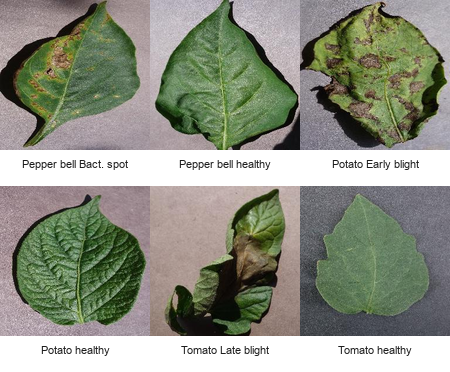
\includegraphics[width=0.68\linewidth]{figures/dataset_samples.png}
\caption{Representative plant leaf images sampled from the local dataset.}
\label{fig:dataset_samples}
\end{figure}

\begin{table}[H]
\centering
\caption{Experimental configuration.}
\label{tab:setup}
\small
\begin{tabular}{l l}
\toprule
Item & Setting \\
\midrule
Framework & TensorFlow/Keras, TensorFlow Lite \\
Backbone & MobileNetV2 \\
Input size & $128 \times 128 \times 3$ \\
Number of classes & 15 \\
Test samples & 2064 \\
Deployment variants & Keras, TFLite FP32/FP16/INT8 \\
Benchmark mode & CPU single-image inference \\
\bottomrule
\end{tabular}
\end{table}

\section{Methodology}
\subsection{Model and Deployment Variants}
The baseline classifier uses MobileNetV2~\cite{sandler2018mobilenetv2}, a lightweight convolutional neural network commonly used for mobile and embedded vision tasks. The trained Keras checkpoint is exported into three TensorFlow Lite formats. Table~\ref{tab:variants} summarizes the role of each evaluated deployment variant.

\begin{table}[H]
\centering
\caption{Model variants evaluated in this study.}
\label{tab:variants}
\small
\begin{tabular}{l l}
\toprule
Variant & Role \\
\midrule
Keras original & Training and quality baseline \\
TFLite FP32 & Edge-compatible baseline \\
TFLite FP16 & Reduced precision deployment \\
TFLite INT8 & Quantized low-latency deployment \\
\bottomrule
\end{tabular}
\end{table}

\subsection{Edge Evaluation Pipeline}
The project implements a reproducible evaluation pipeline. First, the Keras model is evaluated on the test split to obtain accuracy and macro-F1. Second, the trained checkpoint is exported into TFLite FP32, FP16, and INT8 models. Third, each model variant is benchmarked with repeated inference runs. Finally, the results are merged into comparison tables and visualization figures for report generation.

The pipeline is designed to be practical on CPU-only machines. Optional energy and peak-memory tools are used when supported, while unavailable metrics are reported explicitly as \texttt{not\_available} instead of causing execution failure.

\begin{figure}[H]
\centering
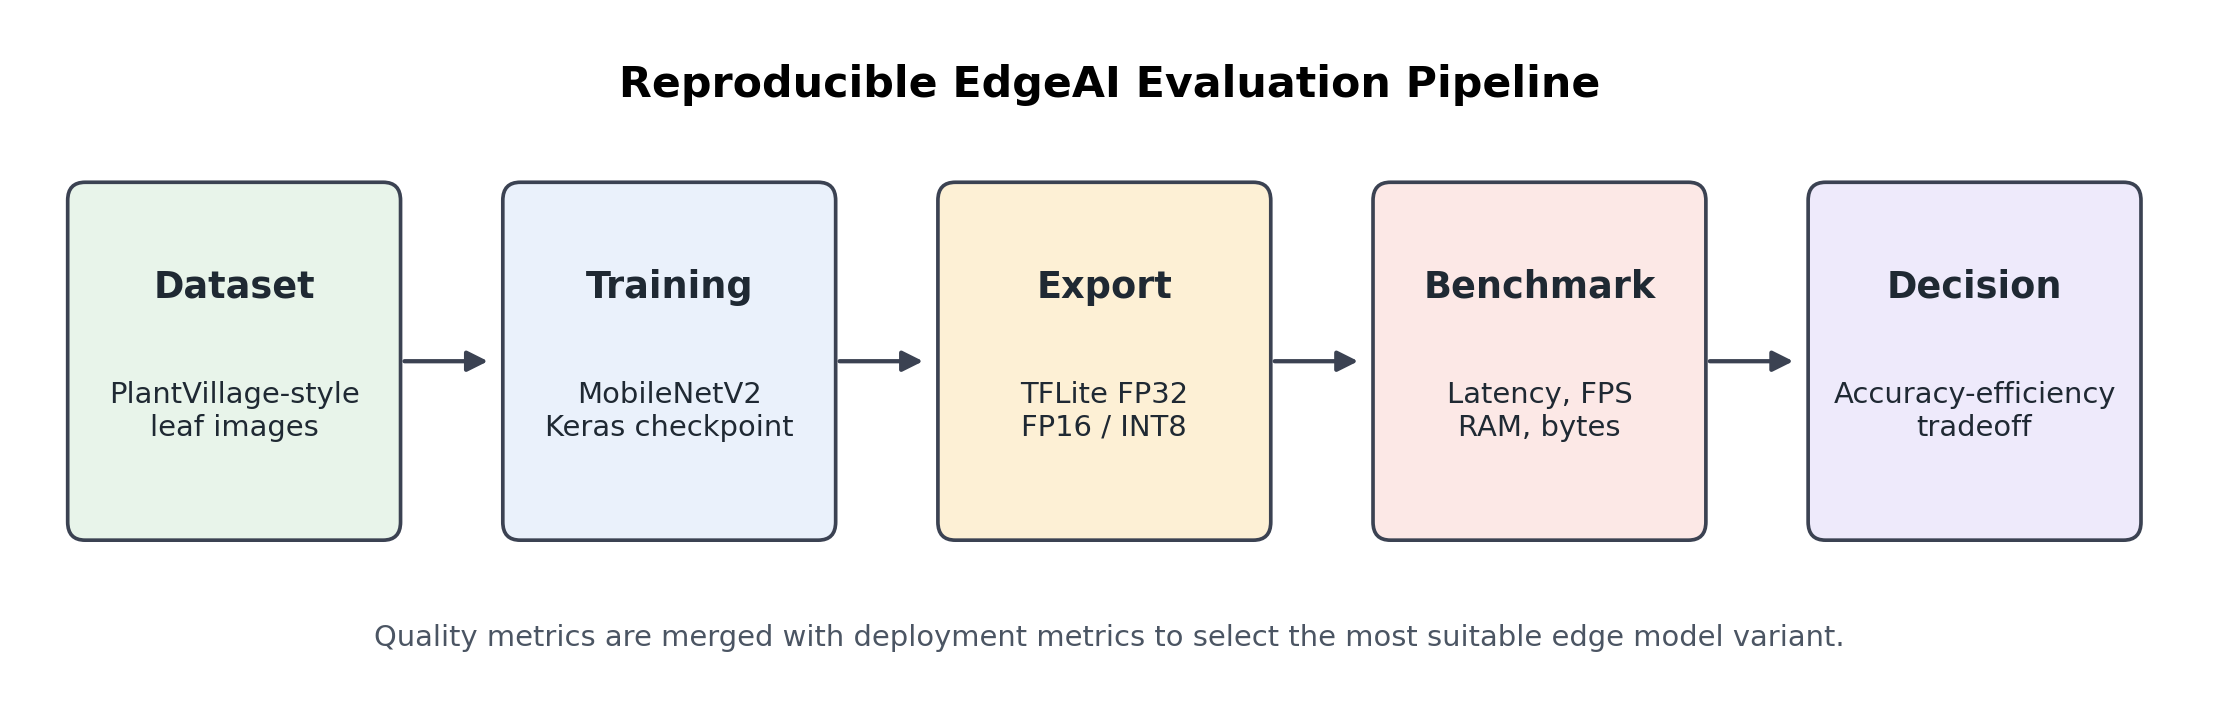
\includegraphics[width=0.86\linewidth]{figures/edge_pipeline.png}
\caption{Reproducible pipeline for evaluating edge deployment tradeoffs.}
\label{fig:pipeline}
\end{figure}

\subsection{Evaluation Metrics}
The evaluation pipeline measures both model quality and edge deployment efficiency. Classification quality is represented by accuracy and macro-F1. Edge efficiency is measured using model size, average latency, p50 and p95 latency, FPS, RAM usage, input/output tensor bytes, and runtime status. Energy and emissions are supported through optional software tools when available on the execution platform.

Latency is measured with \texttt{time.perf\_counter} over repeated inference calls after warmup. Model size is measured directly from the saved checkpoint or TFLite file. RAM usage is measured around the benchmark loop, with a standard-library fallback on macOS/Linux when \texttt{psutil} is unavailable. Communication cost is approximated with input and output tensor byte counts, which is relevant when deciding whether to send raw data, intermediate tensors, or only prediction results.

\section{Experimental Setup}
Experiments were run using the existing project pipeline:

\begin{verbatim}
python scripts/evaluate.py
python scripts/export_tflite.py
python scripts/benchmark.py
python scripts/compare_edge_models.py
python scripts/plot_edge_tradeoffs.py
\end{verbatim}

Each command uses \texttt{config.yaml} as the default configuration file.

The benchmark uses repeated single-image inference after warmup iterations. In the current configuration, each benchmark uses 10 warmup runs and 100 measured inference runs. The reported results are based on the latest generated files under \texttt{results/edge\_benchmark/}. Energy and emissions were not available on the current machine and are therefore reported as unavailable.

All runtime measurements should be interpreted as device-specific measurements. They are valid for comparing variants on the same machine, but absolute latency and FPS may change on a Raspberry Pi, Jetson Nano, mobile phone, or microprocessor-class device. The value of the pipeline is that the same commands can be rerun on the final target device to obtain hardware-specific results.

\section{Results}
The trained classifier reaches 0.9254 accuracy and 0.9163 macro-F1 on the test split. Figure~\ref{fig:confusion_matrix} shows the normalized confusion matrix, which provides a class-level view of prediction behavior. Table~\ref{tab:comparison} summarizes the main edge deployment results. All evaluated deployment variants use the same trained model quality metrics, while their runtime behavior differs significantly.

\begin{figure}[H]
\centering
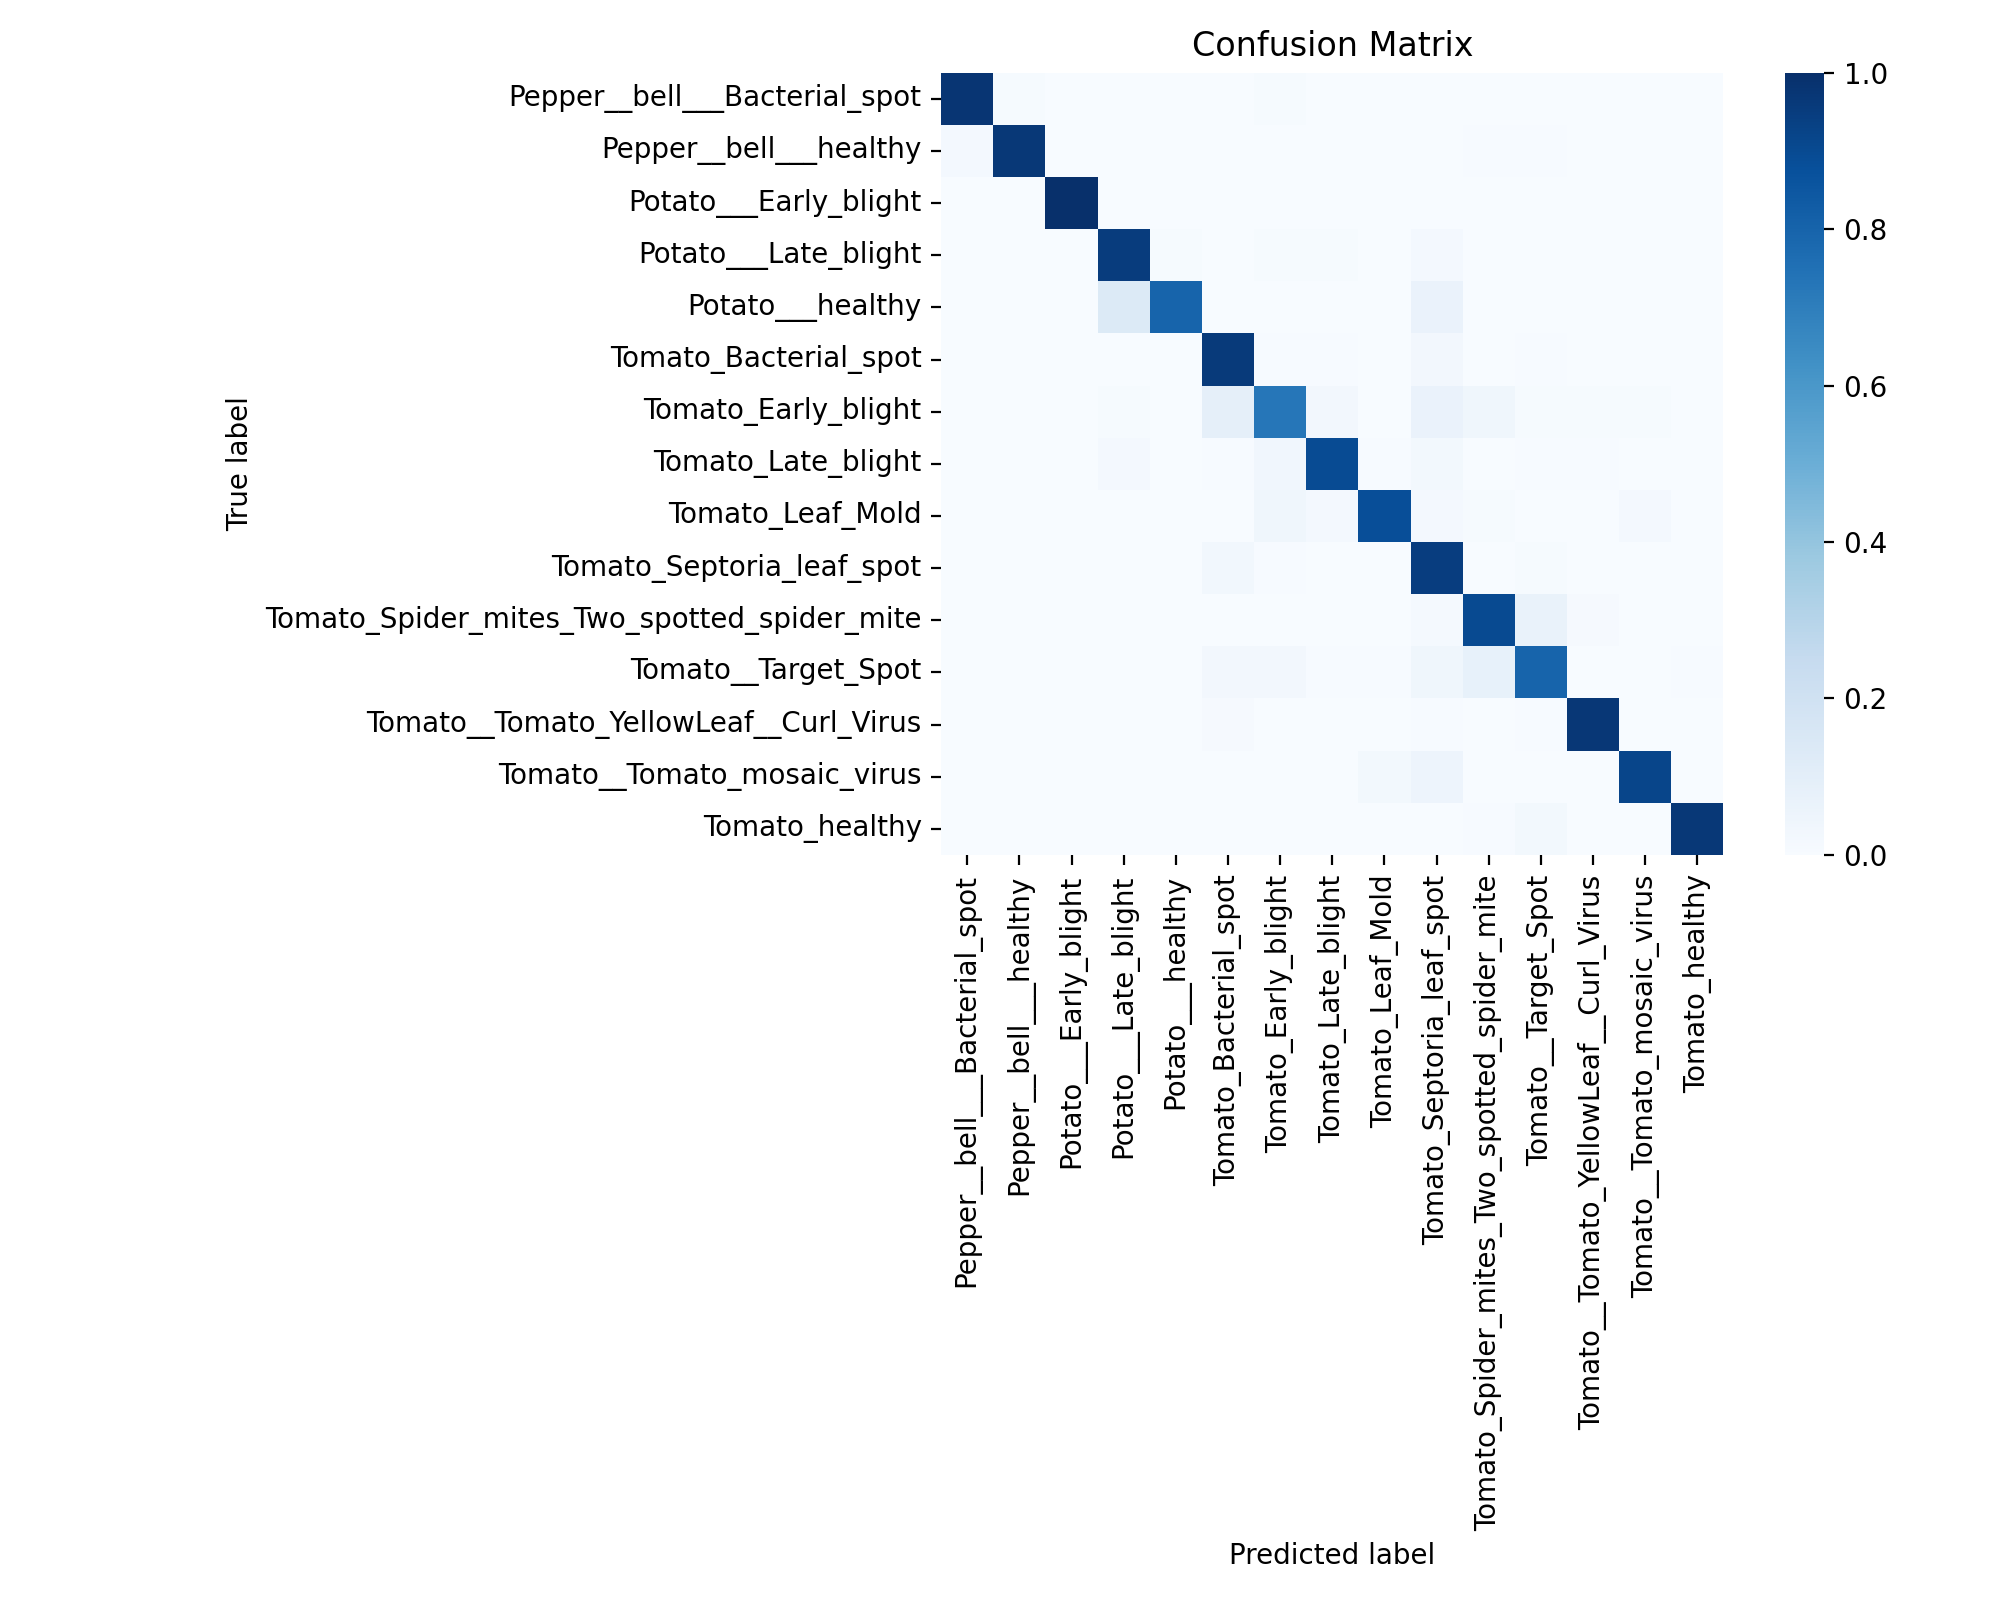
\includegraphics[width=0.56\linewidth]{../results/metrics/confusion_matrix.png}
\caption{Normalized confusion matrix on the test split.}
\label{fig:confusion_matrix}
\end{figure}

\begin{table}[H]
\centering
\caption{Edge deployment comparison of model variants.}
\label{tab:comparison}
\small
\begin{tabular}{l l r r r r r r l}
\toprule
Model Variant & Backend & Accuracy & Macro-F1 & Size MB & Latency ms & FPS & RAM Delta MB & Suitability \\
\midrule
Keras original & Keras & 0.9254 & 0.9163 & 9.3994 & 25.658 & 38.974 & 4.906 & Baseline only \\
TFLite FP32 & TFLite & 0.9254 & 0.9163 & 8.5546 & 2.551 & 391.961 & 0.000 & Strong edge candidate \\
TFLite FP16 & TFLite & 0.9254 & 0.9163 & 4.3445 & 2.505 & 399.259 & 0.000 & Strong edge candidate \\
TFLite INT8 & TFLite & 0.9254 & 0.9163 & 2.6302 & 0.941 & 1062.393 & 0.000 & Strong edge candidate \\
\bottomrule
\end{tabular}
\end{table}

\subsection{Accuracy and Latency Tradeoff}
Figure~\ref{fig:accuracy_latency} shows the accuracy versus average latency. Since all models share the same evaluated accuracy in this experiment, the main difference is inference speed. TFLite INT8 achieves the lowest latency. This result is important for edge applications because latency determines whether inference can be used interactively, for example in a mobile camera workflow or a field inspection tool.

\begin{figure}[h]
\centering
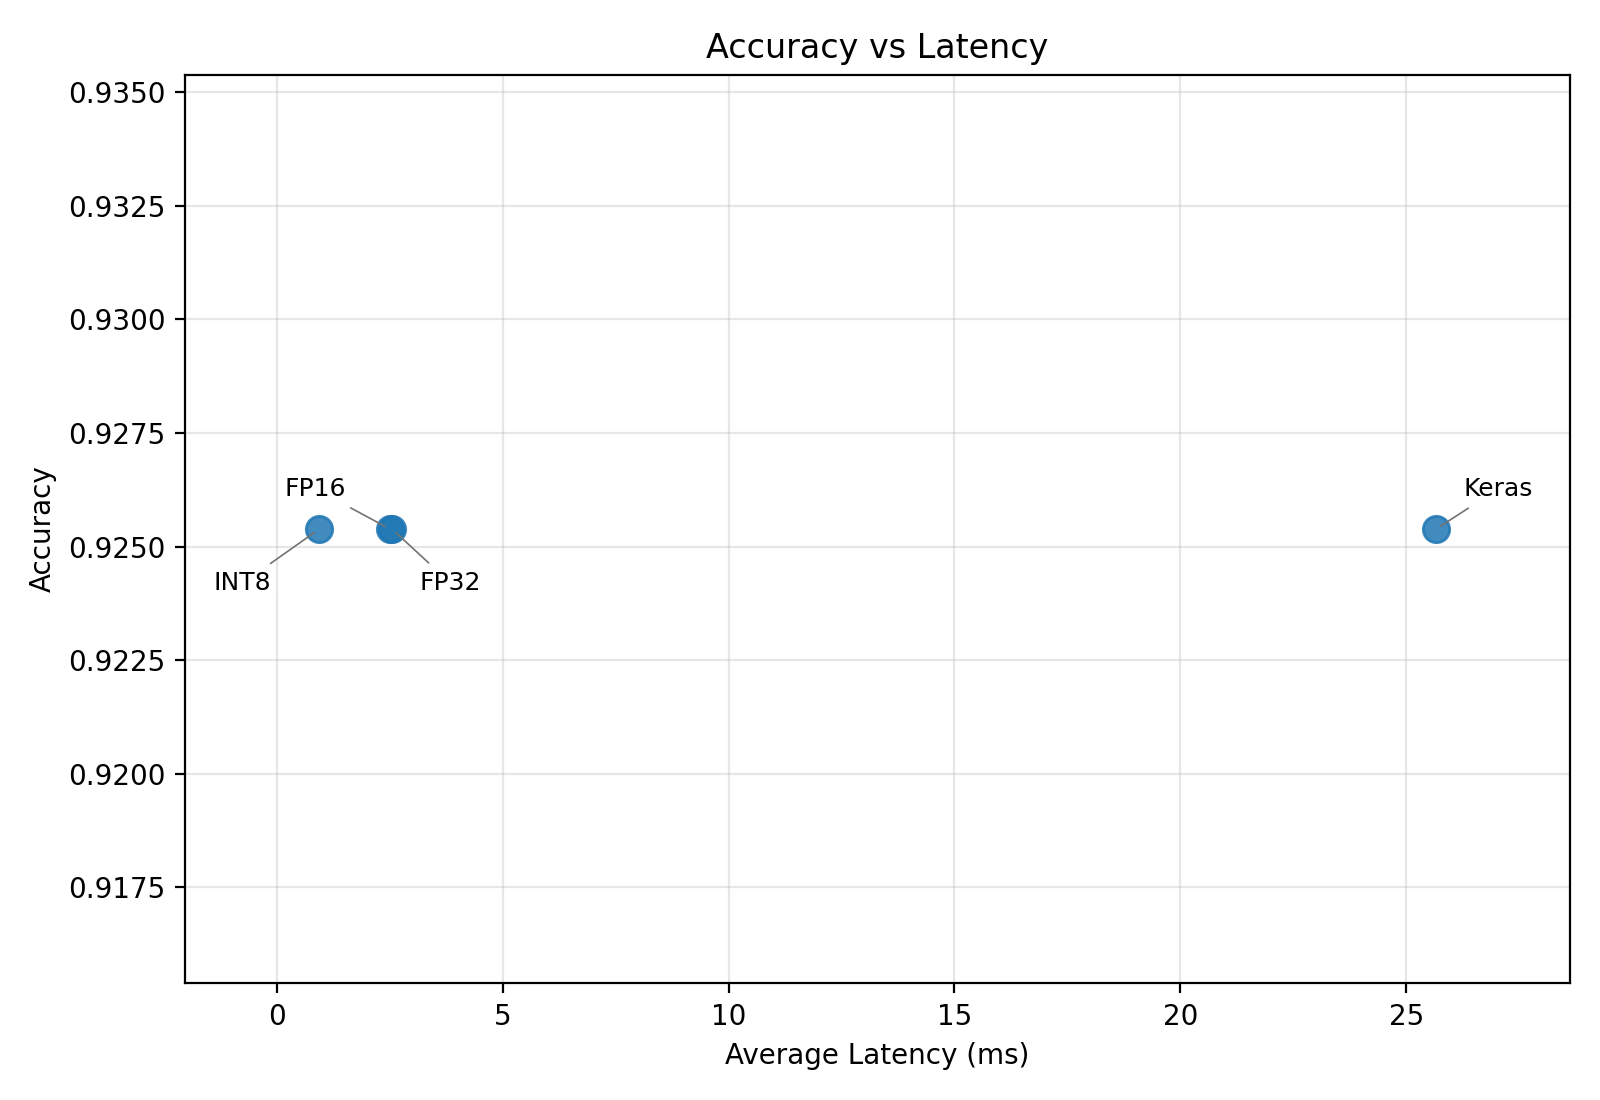
\includegraphics[width=0.56\linewidth]{../results/edge_benchmark/figures/accuracy_vs_latency.png}
\caption{Accuracy versus average inference latency.}
\label{fig:accuracy_latency}
\end{figure}

\subsection{Model Size and Accuracy}
Figure~\ref{fig:size_accuracy} compares model size and accuracy. TFLite FP16 and INT8 significantly reduce model size compared with the original Keras model while maintaining the same reported accuracy. Smaller model files are easier to deploy, update, and store on edge devices. They also reduce communication cost when a model must be transmitted over a network or distributed to many devices.

\begin{figure}[h]
\centering
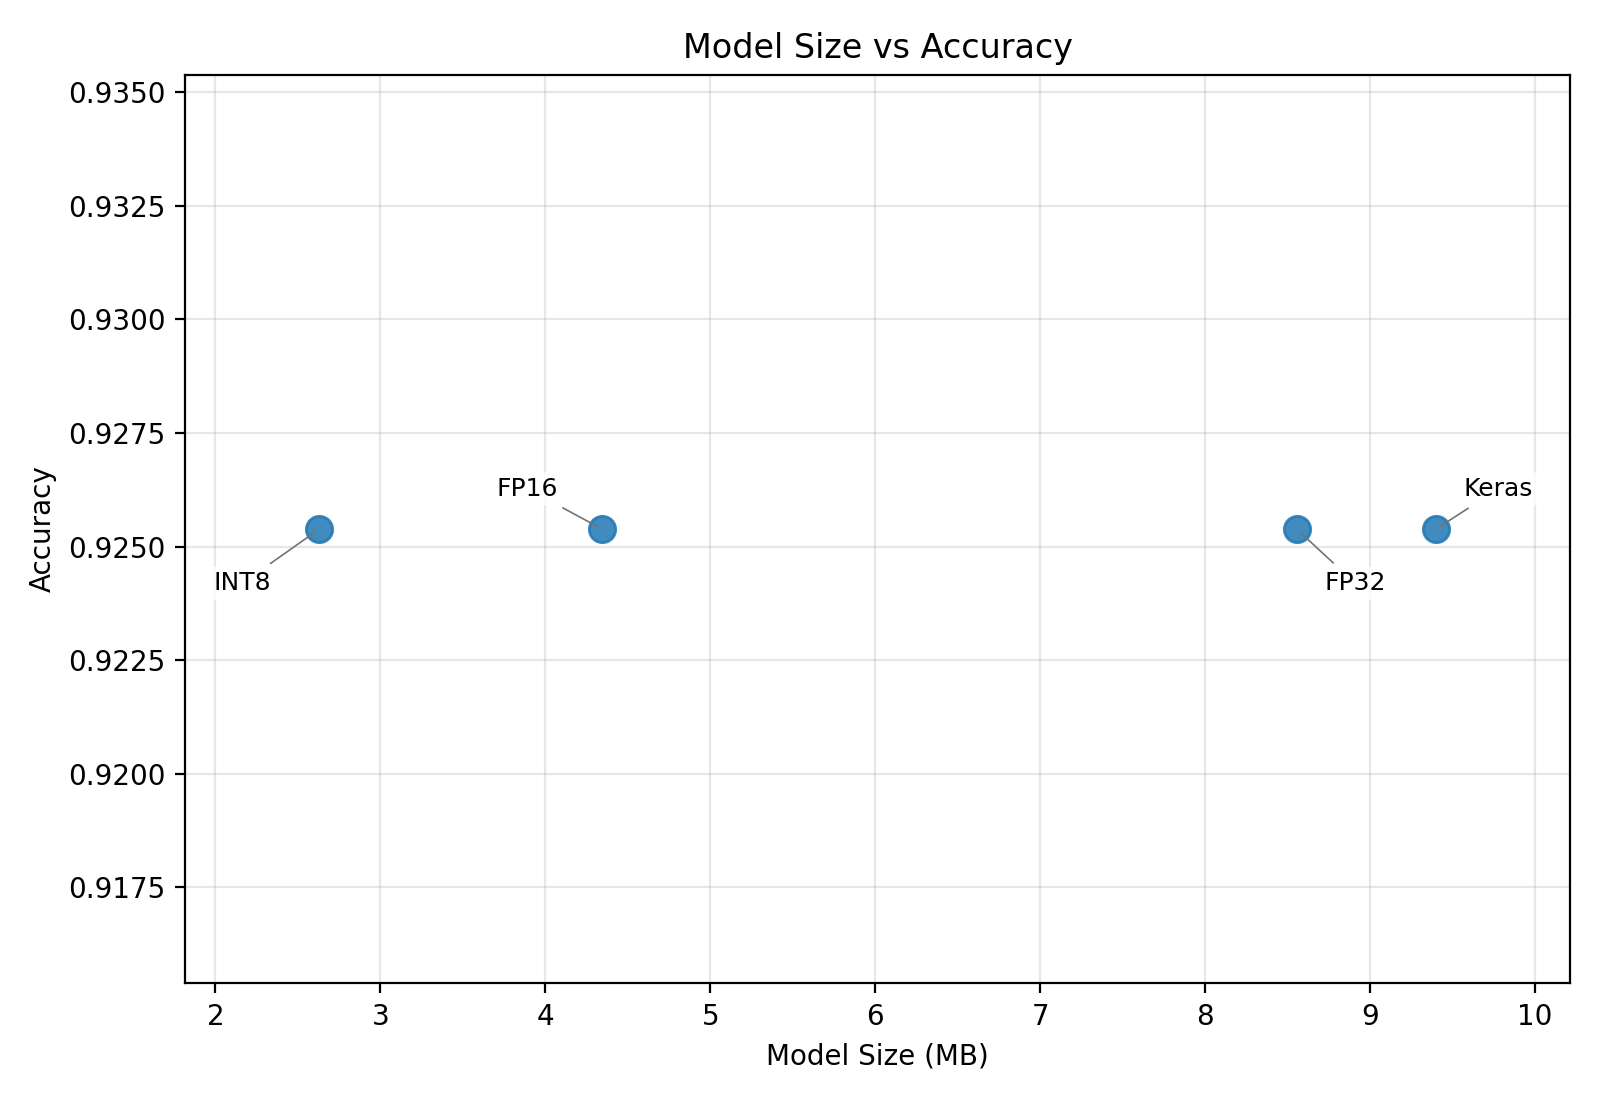
\includegraphics[width=0.56\linewidth]{../results/edge_benchmark/figures/model_size_vs_accuracy.png}
\caption{Model size versus accuracy.}
\label{fig:size_accuracy}
\end{figure}

\subsection{Latency, Throughput, and Memory}
Figures~\ref{fig:latency_size}--\ref{fig:memory} present additional edge efficiency views. The INT8 model has the highest FPS and the smallest model size. The memory comparison shows that the Keras runtime has a higher measured RAM delta, while the TFLite variants are more stable in this benchmark.

\begin{figure}[H]
\centering
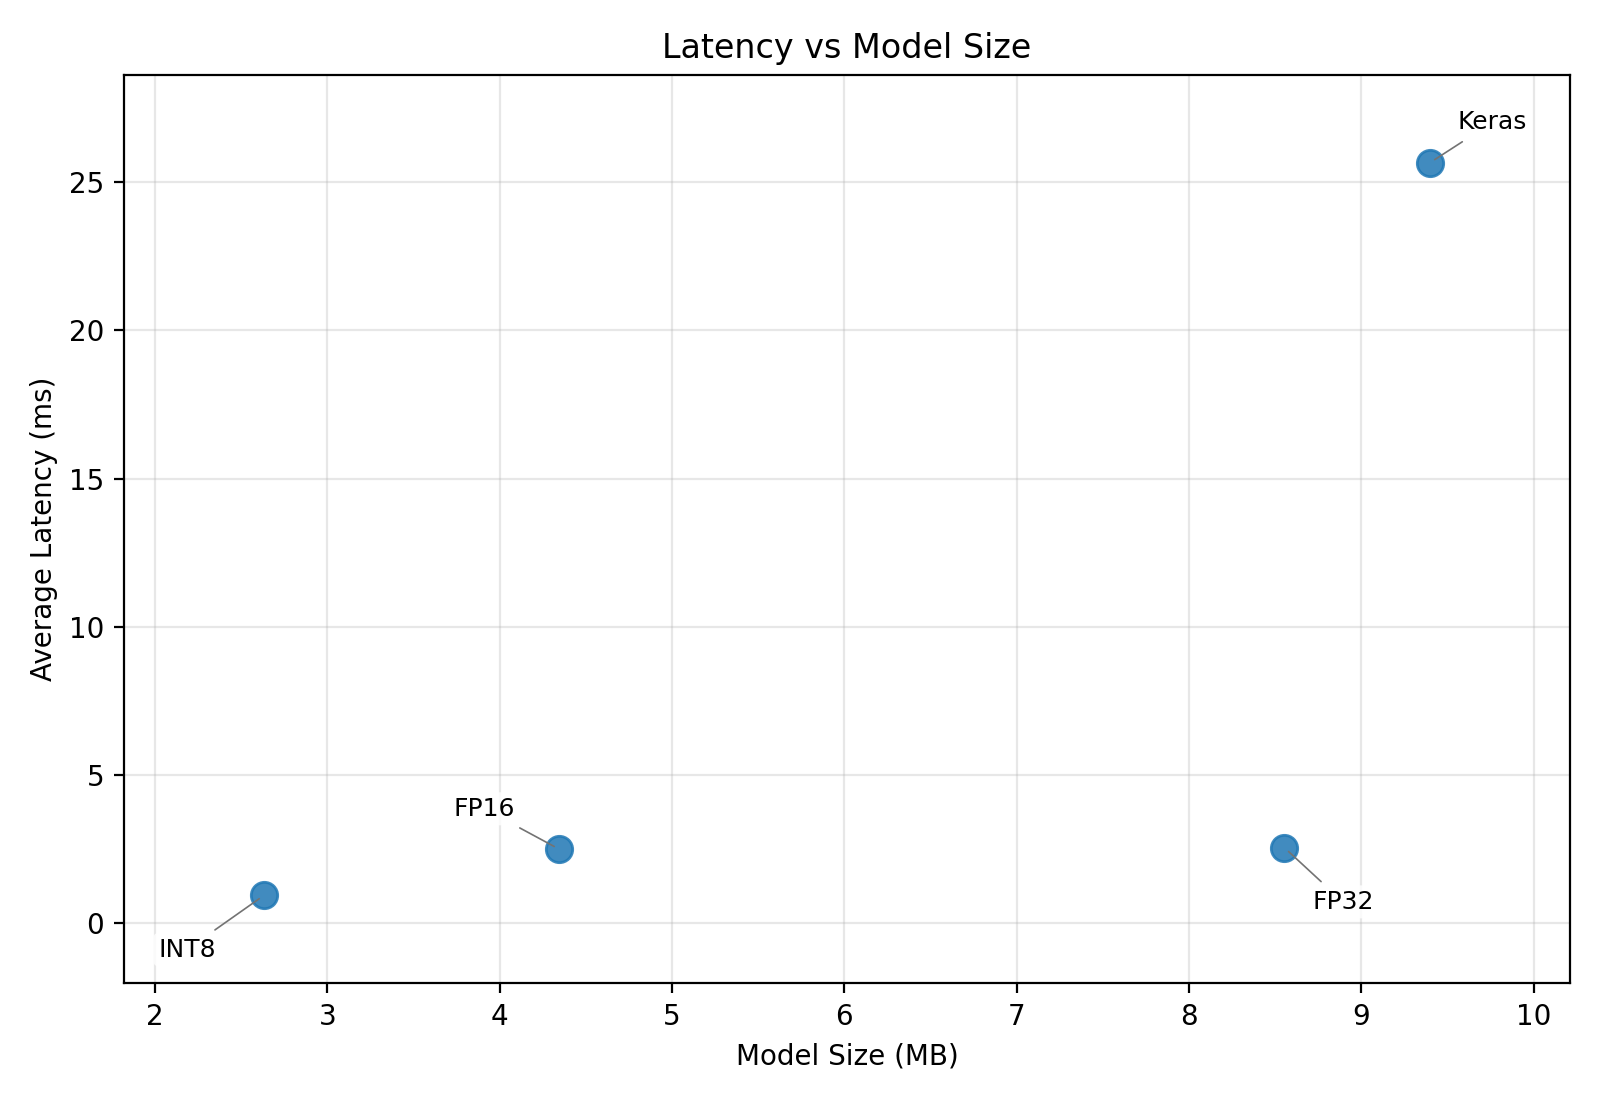
\includegraphics[width=0.56\linewidth]{../results/edge_benchmark/figures/latency_vs_model_size.png}
\caption{Latency versus model size. Lower-left points are preferable for edge deployment.}
\label{fig:latency_size}
\end{figure}

\begin{figure}[H]
\centering
\begin{subfigure}{0.36\linewidth}
    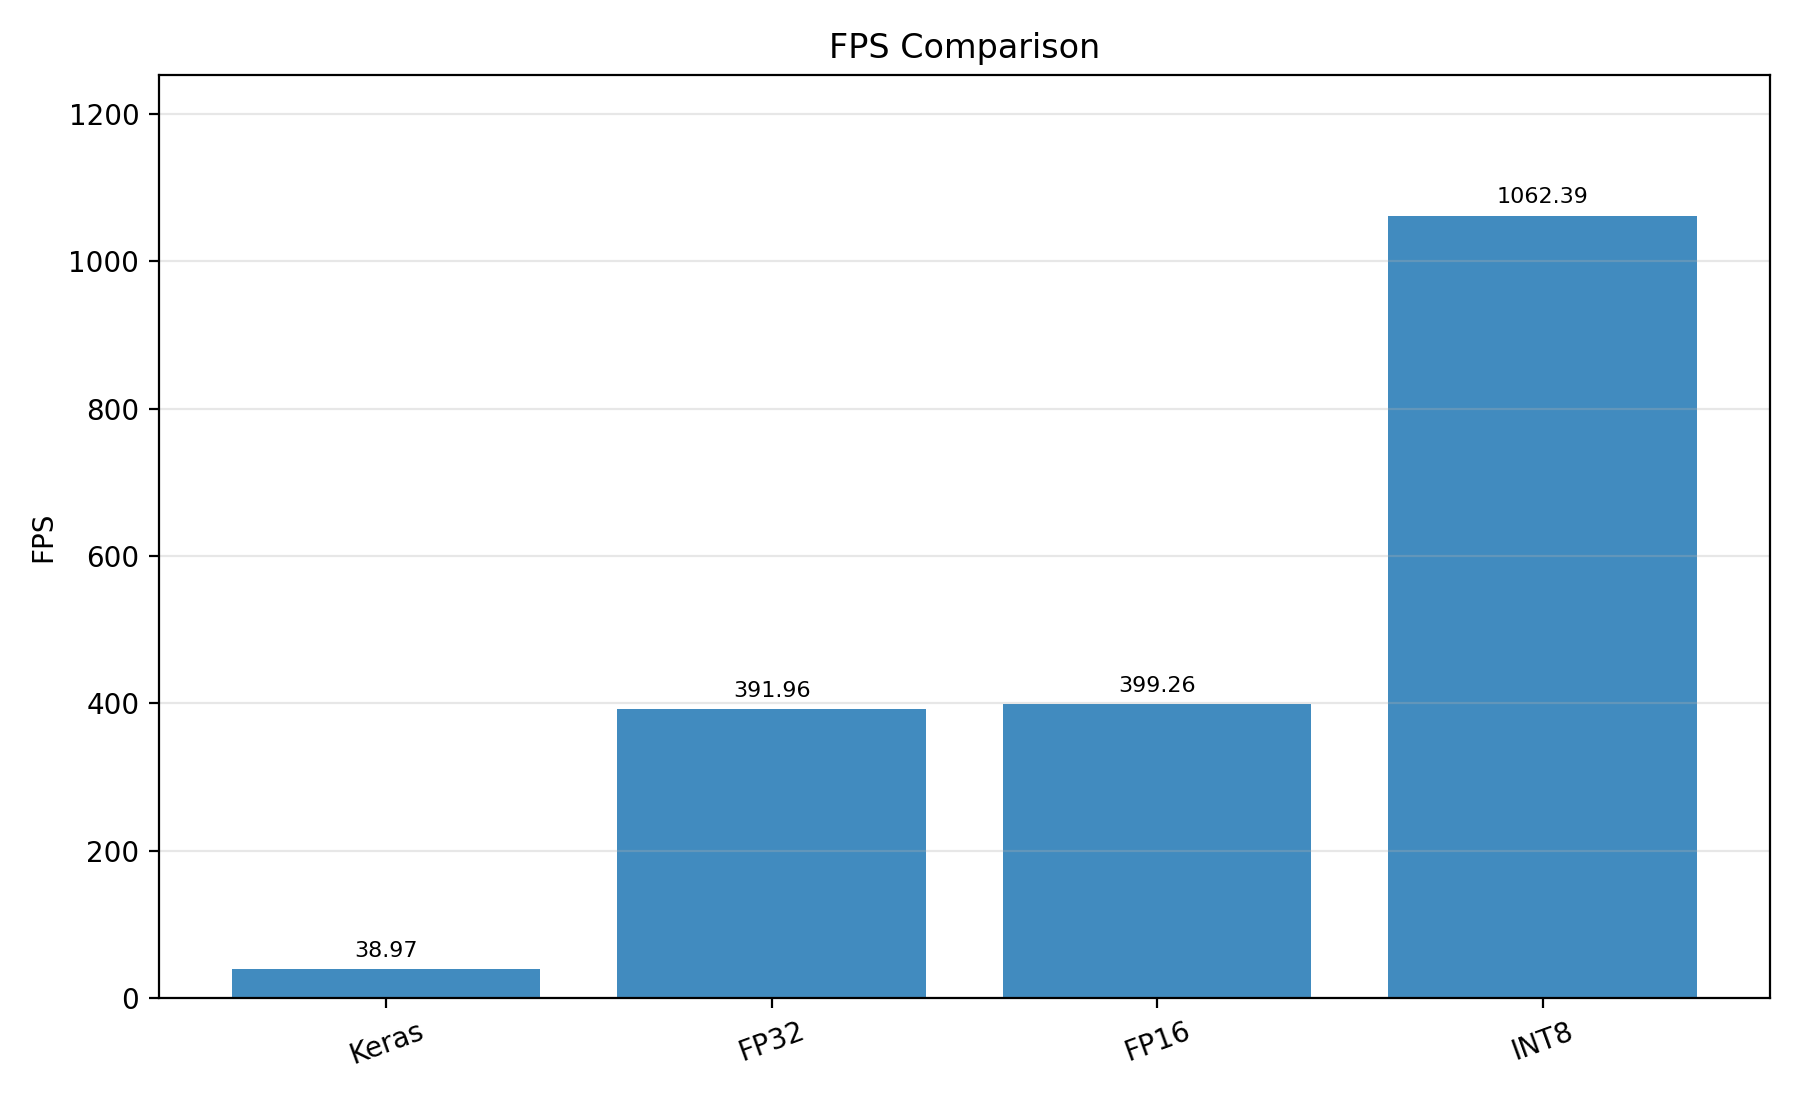
\includegraphics[width=\linewidth]{../results/edge_benchmark/figures/fps_comparison.png}
    \caption{FPS}
    \label{fig:fps}
\end{subfigure}
\hfill
\begin{subfigure}{0.36\linewidth}
    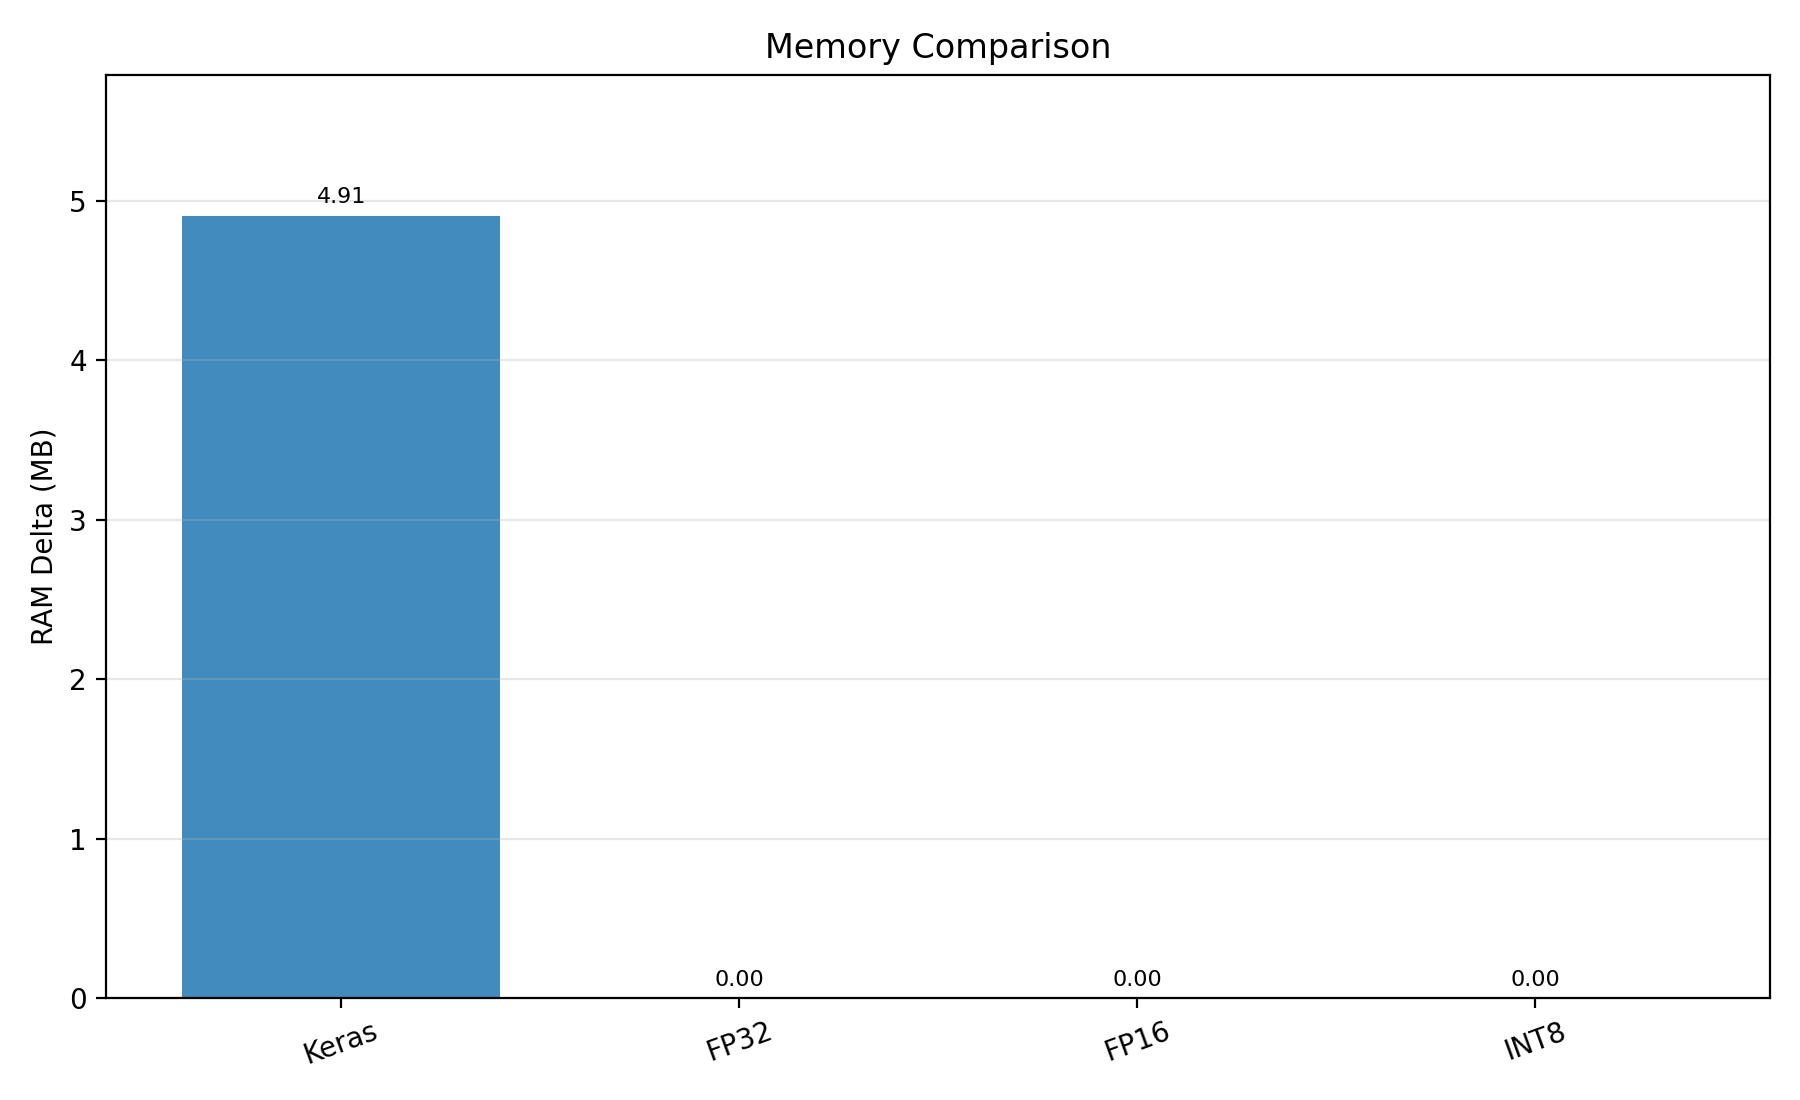
\includegraphics[width=\linewidth]{../results/edge_benchmark/figures/memory_comparison.png}
    \caption{RAM delta}
    \label{fig:memory}
\end{subfigure}
\caption{Throughput and memory comparison for deployment variants.}
\label{fig:throughput_memory}
\end{figure}

\section{Discussion}
The results indicate that TensorFlow Lite is more suitable than the original Keras model for edge deployment. The Keras model is useful as the training and evaluation baseline, but it requires a heavier runtime and has higher latency. TFLite FP32 already provides a large latency improvement, reducing average latency from 25.658 ms to 2.551 ms. TFLite FP16 reduces model size from 8.5546 MB to 4.3445 MB compared with TFLite FP32. TFLite INT8 gives the strongest compression and fastest inference, reaching 2.6302 MB and 1062.393 FPS in the current CPU benchmark.

The comparison also shows that optimization should not be judged by a single metric. FP16 is attractive when storage reduction is important, but in this experiment its latency is similar to FP32 on CPU. INT8 is more aggressive: it reduces both storage and inference time, which makes it the strongest candidate for a constrained deployment. However, quantized models can sometimes reduce accuracy on other datasets or architectures. Therefore, the correct workflow is to evaluate quality and efficiency together after every export.

The INT8 model is therefore the best candidate for a resource-constrained edge device in this experiment. The main limitation is that the current evaluation was performed on a CPU environment rather than a dedicated embedded device. Energy and emissions were also unavailable on the current machine. For final deployment, the same benchmark should be repeated on the target hardware, such as a Raspberry Pi, Jetson Nano, Android phone, or other edge platform.

\section{Conclusion}
This project extends a plant disease classifier into an Edge AI evaluation pipeline. The system now evaluates both classification quality and deployment efficiency. Among the tested variants, TFLite INT8 achieves the best accuracy-efficiency tradeoff, with the smallest model size, lowest latency, and highest FPS. The pipeline is reproducible and can be used to compare future pruned, distilled, or combined optimization models.

\begin{thebibliography}{1}
\bibitem{sandler2018mobilenetv2}
M. Sandler, A. Howard, M. Zhu, A. Zhmoginov, and L. Chen, ``MobileNetV2: Inverted residuals and linear bottlenecks,'' in \emph{Proc. IEEE/CVF Conference on Computer Vision and Pattern Recognition}, 2018.

\bibitem{tflite}
TensorFlow, ``TensorFlow Lite: ML for mobile and edge devices,'' 2026. [Online]. Available: \url{https://www.tensorflow.org/lite}
\end{thebibliography}

\end{document}
